\documentclass[10pt,a4paper]{article}
\usepackage[T1]{fontenc}
\usepackage[scaled]{helvet}
\usepackage{cite}
\usepackage{url}
\usepackage{graphicx}
\usepackage{listings}
\usepackage{float}
\usepackage{amsmath}
\usepackage{listings}
\usepackage{color}
 
\definecolor{dkgreen}{rgb}{0,0.6,0}
\definecolor{gray}{rgb}{0.5,0.5,0.5}
\definecolor{mauve}{rgb}{0.58,0,0.82}
\lstset{ %
  language=Octave,                % the language of the code
  basicstyle=\footnotesize,           % the size of the fonts that are used for the code
  numbers=left,                   % where to put the line-numbers
  numberstyle=\tiny\color{gray},  % the style that is used for the line-numbers
  stepnumber=1,                   % the step between two line-numbers. If it's 1, each line 
                                  % will be numbered
  numbersep=5pt,                  % how far the line-numbers are from the code
  backgroundcolor=\color{white},      % choose the background color. You must add \usepackage{color}
  showspaces=false,               % show spaces adding particular underscores
  showstringspaces=true,         % underline spaces within strings
  showtabs=false,                 % show tabs within strings adding particular underscores
  frame=none,                   % adds a frame around the code
  rulecolor=\color{black},        % if not set, the frame-color may be changed on line-breaks within not-black text (e.g. commens (green here))
  tabsize=4,                      % sets default tabsize to 2 spaces
  breaklines=true,                % sets automatic line breaking
  breakatwhitespace=false,        % sets if automatic breaks should only happen at whitespace
  keywordstyle=\color{blue},          % keyword style
  commentstyle=\color{dkgreen},       % comment style
  stringstyle=\color{mauve},         % string literal style
  escapeinside={\%*}{*)},            % if you want to add LaTeX within your code
  morekeywords={*,...}               % if you want to add more keywords to the set
}
\usepackage{amssymb}
\usepackage{fancyhdr}
\usepackage{lastpage}
\floatstyle{boxed} 
\restylefloat{figure}
\renewcommand*\familydefault{\sfdefault}
\title{Efficent Retrevial from Data Structures}
\author{David Lynch - david.lynch@raglansoftware.com }
\begin{document}
\maketitle
\begin{abstract}
In this article, we look at two data-structures that facilitate efficient retrieval given an explicit key. This style of data-structure is commonly used in situations where we desire optimized look-up. For example, maintaining a dictionary of definitions of a particular word, and then searching  for definitions by that word. We consider hash tables and binary search trees as two relatively simple structures that aim for efficiency in retrieval. 
\end{abstract}
\section{Introduction}
This article is somewhat heavy in theory and even when code is provided, it is quite terse. My suggestion for handling this paper is to first read right through. At every point, ensure that you can build concrete examples of each data structure. Pay particular attention to edge cases, especially if these cases cause the running time of some operation to break down. Lastly, I encourage you to write your own Hash Table implementation in Java, followed by your own BST implementation. Only when you are comfortable with all of this would I suggest you take a look at the further reading part of each section, with the exception of using the MIT-Open-courseware video lectures to compliment this material. Beware that we are only skimming through both of these data-structures, and the materials described consider each structure in much more detail. I would only venture here if you're really interested, or to hammer home your understanding. There is enough in this article to do very well any related exam question. 
\section{Hash Tables}
A hash table is an interesting data structure for a number of reasons. Firstly, you'll see them where you might want to maintain a keyed list of data. The upper bound $\theta(1)$ nature of the retrieval is very desirable the for applications, such as dictionaries, that require quick mapping of values to other values. More interestingly, due to space constraints performance of hash tables may not remain constant for the duration of its existence. This makes for a simple example of a data structure that requires work to maintain its {\it feature} property. Searching for an element in a hash table has an upper bound of $\Theta(n)$ but given reasonable assumptions about the hash table, retrieval can be expected at $O(1)$. A hash table generalizes the simpler notion of an array by using direct addressing as a means to implement an explicit key. When the number of keys stored is small relative to the number of possible keys, hash tables are an effective alternative to maintaining an complimentary array of direct addresses. Conceptually, the array index is computed from the {\bf key} by applying a {\bf hash function} to the key. When {\bf collisions} occur in a hash table {\bf chaining} is used to resolve the key-pair mapping. 
\subsection{Direct Address Tables}
When the {\it universe} of possible keys is small, direct-address tables are useful. Each element has a key from the universe $U={0,1...,m-1}$ where $m$ is not too large by some measure and the function $f(k)$ enforces the rule that no two elements have the same key. In other words for any key $k$ there is no key $k'$ in the universe of keys $U$ whereby $k=k'$. Direct addressing implementation is relatively trivial. Figure \ref{diraddr} illustrates direct addressing. 

\begin{figure}
\caption{Direct address tables \cite{INTROALG}}
\begin{center}
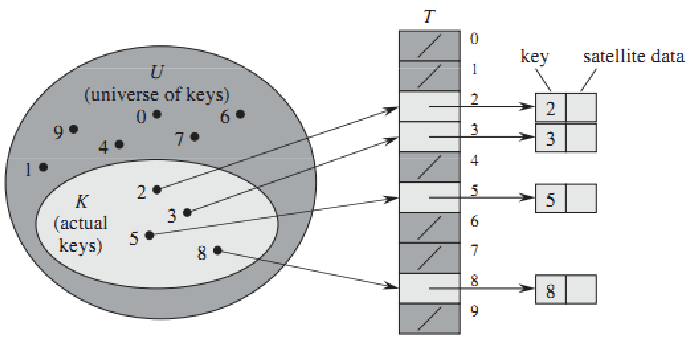
\includegraphics[scale=0.43]{../images/directaddtables.png}
\label{diraddr}
\end{center}
\end{figure}
\subsection{Hash Tables}
If $U$ is sufficiently large, storing a table $T$ of size $|U|$ may be impractical, or even impossible. Also, the set of keys $K$ that is actually stored may be so small relative to $U$ that most of the space allocated for $T$ would be wasted. For large $U$ therefore, direct address tables are not space efficient. When the set of keys $K$ stored in a dictionary is much smaller than the universe $U$ of all possible keys, a hash table, which manages key collisions is much more space efficient. In fact we can reduce the storage requirement to $O(|K|)$ while maintaining the $O(1)$ access time property on average. With direct addressing element with key $k$ is stored in slot $h(k)$ where $h$ key is a simple mapping. With hashing the function $h(k)$ is a hash function $H : U -> {0,1...m-1}$. Collisions in the hash space are minimized by clever design of H and and keeping $m << U$. Figure \ref{hashtable} shows this diagrammatically, and also shows how each slot degrades to a linked list in the presence of collisions. 
\begin{figure}
\caption{A hash table with chaining \cite{INTROALG}}
\begin{center}
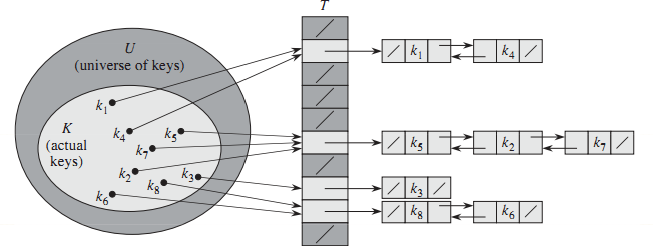
\includegraphics[scale=0.43]{../images/hashtable.png}
\label{hashtable}
\end{center}
\end{figure}
\subsection{Chaining}
Given a hash table $T$ with $m$ slots that stores $n$ elements {\bf load factor}  $\alpha$  for $T$ is defined as $n/m$ or the average number of elements stored in a chain. Retrieval performance degrades to that of a linked list, but insertion stays at constant time. The overall average-case performance of a hash table with chaining depends on how well the hash function distributes the set of keys to be stored among the $m$ available slots. If we assume that any given element is equally likely to hash to any of the $m$ slots, independently of where other elements have already hashed, then we assume {\bf simple, uniform hashing}. In a hash table in which collisions are resolved by chaining, a search takes an average time of  $O(1+\alpha)$.
\subsection{Hash Functions}
A good hash function satisfies the simple uniform hashing assumption. It is very difficult to implement without {\it a priori} knowledge of the probability distribution of the drawing of keys. In practice we use heuristic techniques to create hash functions that perform well. In this case qualitative information about key distribution may be very useful. A good approach derives the hash value independently of any patterns that might exist in the data. Some applications of hash functions might require stronger properties than are provided by simple uniform hashing. We might get keys that are close to yield hash values that are far apart, or vice versa. Most hash functions assume the universe of keys to be the natural set of numbers N. If keys are not natural numbers we can find a way of interpreting them as such. 
\subsubsection{The Division Method}
Using this method a key $k$ is mapped to one of its $m$ slots by taking the remainder of $k$ divided by $m$ so that $h(k) = k mod (m)$. This can be performed in a single division and as such is quite fast. For example, if the hash table has a size of $m=12$ and the key is $k=100$ then $h(k)=4$. Certain choices of m are undesirable. The case where $m$ is a power of 2 needs to be avoided, since if $m=2^p$ then $h(k)$ maps directly to the   the $p$ lower order bits of $k$. Unless we know for sure that all lower-order $p$-bit patters are equally likely, we are better designing the hash function to depend on all the bits of the key, rather than a sub-set.
\newline\newline
A prime not too close to an exact power of two is often a good choice for $m$. Suppose we wish to allocate a hash table with $n=2000$ character strings, where a character has 8-bits. We are happy with the cost of examining an average of 3 elements in an unsuccessful search. We choose $m=701$ in this case because 701 is prime near $2000/3$ but not near every power of 2. Our hash function becomes $h(k) = k mod 701$

\subsection{Further Reading}
The MIT Open-Courseware lecture at \cite{HASHTABLE} covers most of the ground we have covered above, with a slightly more detailed treatment on what makes a good hash function. It also includes some details on the multiplication method. Outside hash tables themselves, MD5 is well worth a look, see the RFC here \cite{MD5}. This hash function is commonly used in verifying the integrity of data, and is slightly orthogonal to the functions commonly used by hash tables as data structures. However, it is practical use makes it well worth the read. 

\section{Binary Search Trees}
Operations on binary search trees take time proportional to the height of the tree. For a complete binary tree with $n$ nodes operations run in $O(n log n)$ time, but if the tree is a linear collection of $n$ nodes it is $O(n)$ time. We can capture both cases by generalizing to $O(h)$ running time, where $h$ is the height of the tree. 
\newline\newline
A binary search tree is a {\bf binary tree} with some extra properties. Each node in the tree contains a {\bf key}, {\bf satellite data} and attributes {\bf left},{\bf right} and {\bf parent} as pointers to other nodes in the tree. The keys in a binary search tree are always stored in a way that satisfies the {\bf binary search tree property} which is defined as follows.
\newline\newline
Let $x$ be a node in a binary search tree. \\
If $y$ is a node in the left sub-tree of $x$, then $y.key <= x.key$. \\
If $y$ is a node in the right sub-tree of $x$, then $y.key>=x.key$.
\newline\newline
Note that for the same overall set of keys, insertion order into the tree is significant in the resulting shape. Figures \ref{bstupright} and \ref{bstfull} illustrate this, more about this in the further reading section. For now, we focus on how to construct, search through and maintain the structure. 

\begin{figure}
\caption{Upright form of the BST tree for {[2,5,5,6,7,8]} - $h=5$ }
\begin{center}
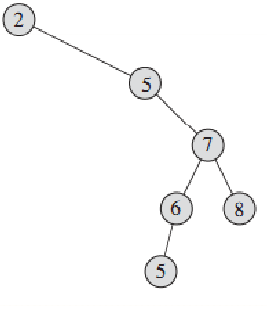
\includegraphics[scale=0.43]{../images/bstupright.png}
\label{bstupright}
\end{center}
\end{figure}

\begin{figure}
\caption{Full form of the BST tree for {[2,5,5,6,7,8]} - $h=3$}
\begin{center}
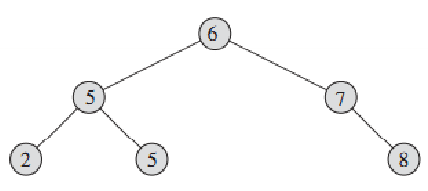
\includegraphics[scale=0.43]{../images/bstfull.png}
\label{bstfull}
\end{center}
\end{figure}


\begin{figure}
\caption{Tree Walking and Search}
\begin{center}
\begin{lstlisting}
INORDER-TREE-WALK(x)
if x != NIL
  INORDER-TREE-WALK(x.left)
  print x.key
  INORDER-TREE-WALK(x.right)
\end{lstlisting}

\begin{lstlisting}
TREE-SEARCH(x, k)
if x==NIL or k==x.key
  return x
if k<x.key
  return TREE-SEARCH(x.left, k)
else
  return TREE-SEARCH(x.right, k)
\end{lstlisting}


\begin{lstlisting}
ITERATIVE-TREE-SEARCH(x, k)
while x.left!=NIL and k!=x.key
  if k<x.key
     x=x.left
  else  
     x=x.right
return x
\end{lstlisting}
\label{walkandsearch}
\end{center}
\end{figure}


\subsection{Tree Traversal}
The BST property allows printing of all keys in a binary search tree in {\bf sorted} order by walking the tree {\bf in-order}. This kind of traversal entails first printing the key of the root between printing the values in the left sub-tree and those in the right sub tree. {\bf Pre-order} traversal is when the root is printed before values in either sub-tree. Lastly, {\bf post-order} traversal prints the root after the values in each of the sub-trees. An in-order tree walk takes $O(n)$ time since after the initial call the procedure calls itself exactly twice, or once for each node. 
\newline\newline
Figure \ref{walkandsearch} shows an in-order walk, and two forms of tree search, one recursive and one iterative. We can see that the binary search tree property not only enables retrieval in $O(h)$ time but facilitates us in finding particularly elegant operation implementations. To search for a particular key we simply navigate the tree from the root. If the key of the current node, starting at the root, is less than the root itself, then we proceed to the left sub-tree, otherwise, as the BST property states, we progress to the right sub-tree. This operation is $O(h)$ because if we enforce this rule, the maximum number of iterations we will need is equal to the number of levels in the tree.  


\begin{figure}
\caption{Useful helper operations on Binary Search Trees.}
\begin{center}
\begin{lstlisting}
TREE-MINIMUM(x)
while x.left != NIL
  x = x.left
return x
\end{lstlisting}

\begin{lstlisting}
TREE-MAXIMUM(x)
wile x.right != nil
  x = x.right
return x
\end{lstlisting}

\begin{lstlisting}
# Given a node, find the successor in the sorted order
# that is determined by an in-order tree walk
TREE-SUCCESSOR(x)
if x.right != NIL			   # If there are keys greater than this
  return TREE-MINIMUM(x.right) # Must be the least node that
  							   #  is greater than this
y = x.parent				   # Trailing pointer 
while y!=NIL and x==y.right	   # In the case of equality,
							   #  find the last inserted node 
	x = y
	y = y.parent
return y
\end{lstlisting}
\label{helperbst}
\end{center}
\end{figure}

\subsection{Tree Modification}
Since the BST is optimised for retrieval, we are willing to pay some up front cost in logical complexity of the tree modification operations. To insert into a BST we first start at the root of the tree with a pointer $x$ tracing a simple path downwards looking to replace NIL with the node we wish to insert which we will denote as $z$. The listing for the insertion is shown in figure \ref{bstinsert}. The trailing pointer $y$ is the parent of $x$ and we are required to track it since by the time we hit NIL we need a pointer to the parent of NIL so that we can add the new node to the parents' children. Remember, NIL is nothing, and therefore we cannot get from NIL back to a parent. Each of the pointers $x$ and its parent $y$ moves down the tree as if we were conducting a search. As a result, the insertion operation is also a $O(h)$ running time operation. 
\newline\newline
BST deletion is much more complex, as there are a number of edge cases we need to consider. Firstly, we introduce the {\it TRANSPLANT} operation detailed in the first code listing of \ref{bstdeletion}. This operation facilitates the replacement of one sub-tree as a child of its parent with another sub-tree. Specifically {\it TRANSPLANT} replaces the sub-tree rooted at node $u$ with the sub-tree rooted at node $v$, making node $u$'s parent become node $v$ parent and $u$ parent ends up having $v$ as its appropriate child. 
\newline\newline
When we come to deletion, which is listed in \ref{bstdeletion} we need to consider 4 cases. Cases $a$ and $b$, whereby we have only one child in the node that is to be delete is illustrated by figure \ref{bstdelab}. In this case, we simply shift the available child node up into the position of the node to be deleted. Case $c$ is illustrated by figure \ref{bstdelc} covers the scenario whereby the successor of $z$ is in its immediate right tree and the left child of the successor is NIL. In this case we can transplant $y$ into the old slot occupied by $z$, maintaining the old right sub-tree of $y$ and setting the left child of $y$ to be that of $z$'s left child. The final case is $d$ illustrated by figure \ref{bstdeld}. The successor to $z$ in this case lies somewhere on the left side of the right sub-tree of $z$. In this case, the minimum needs to be transplanted into $z$'s old position and $y$ made the parent of the right child of $z$. 

\begin{figure}
\caption{Deletion with NIL left or right sub-trees respectively}
\begin{center}
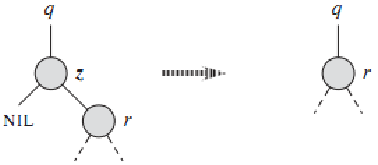
\includegraphics[scale=0.43]{../images/bstdeletea.png}
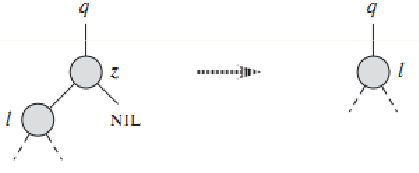
\includegraphics[scale=0.43]{../images/bstdeleteb.png}
\label{bstdelab}
\end{center}
\end{figure}

\begin{figure}
\caption{Deletion with right successor that has a NIL left node}
\begin{center}
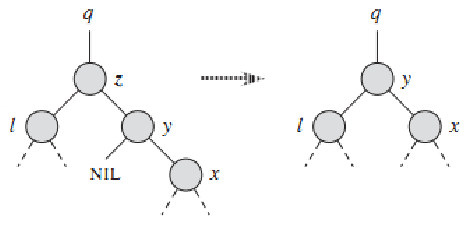
\includegraphics[scale=0.43]{../images/bstdeletec.png}
\label{bstdelc}
\end{center}
\end{figure}

\begin{figure}
\caption{Deletion where successor is somewhere to the right of the left node subtree.}
\begin{center}
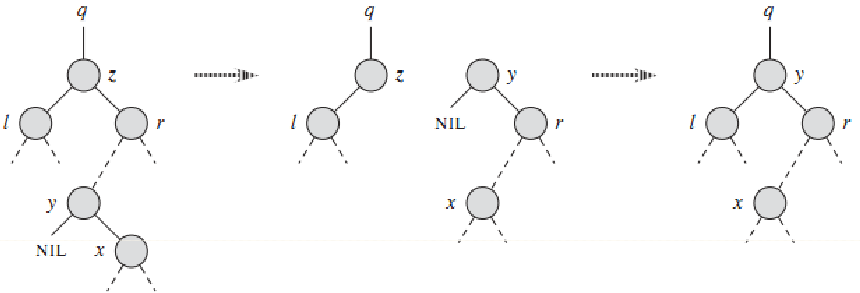
\includegraphics[scale=0.40]{../images/bstdeleted.png}
\label{bstdeld}
\end{center}
\end{figure}

\begin{figure}
\caption{Insertion into a Binary Search Tree}
\begin{center}
\begin{lstlisting}
TREE-INSERT(T, z)
y=NIL     			# trailing pointer
x=T.root  			# current node 
while x!=NIL		
  y=x				# parent becomes current node
  if z.key <x.key	
    x=x.left		# advance current pointer
  else
    x=x.right
x.p=y				# Found nil, set x's parent to y				
if y==NIL			# Tree was empty to start with
  root=z	
elsif z.key<y.key
  y.left=z			# Ensure z gets placed as a child of y
else
  y.right=z
\end{lstlisting}
\label{bstinsert}
\end{center}
\end{figure}



\begin{figure}
\caption{Deletion from a binary search tree}
\begin{center}
\begin{lstlisting}
# Replace a node u with a node v
# v will assume all the connections of u while 
# maintaining the BST property relative to u's parent
TRANSPLANT(T,u,v)
if u.p==NIL			# This is the root, replace immediately
	T.root = v
elsif u=u.p.left	# At left sub-tree, insert at left of parent
	u.p.left=v
else				# At right sub-tree, insert at right of parent
	u.p.right=v
if v!=NIL			# Obliterate u by making v the new connection from u
	v.p=u.p
\end{lstlisting}
\begin{lstlisting}
TREE-DELETE(T,z)
if z.left==NIL					# If z has no left, replace z with 
								# its right child
	TRANSPLANT(T,z,z.right)
elseif z.right=NIL				# Otherwise if z has a left but no right, 
	TRANSPLANT(T,z,z.left)		# replace z with its left child	
else 							# If z has a left and a right child
	y=TREE-MINIMUM(Z.right)		
	if y.p!=z					# Right child contains its successor 	
		TRANSPLANT(T,y,y.right) # Shift y up into z's slot
		y.right=z.right     	# Add z's old right to y
		y.right.p=y             # Make y z's old rights' parent
	TRANSPLANT(T,z,y)			# Reconcile the left child 
	y.left=z.left				
	y.left.p=y
\end{lstlisting}
\label{bstdeletion}
\end{center}
\end{figure}

\subsection{Further Reading}
We showed earlier on that the order of insertion into a binary search tree has a bearing on the performance of the search algorithm. There are a number of ways to mitigate against the degradation of search to $O(n)$. One way, is to randomize the building of the binary search tree. If each of the $n!$ permutations of this random build is equally likely, then we can show that the expected height of a randomly built binary search tree is $O(lg n)$. This is discussed in section 12.4 of \cite{INTROALG}. Another optimization is covered in chapter 13 of \cite{INTROALG}. A red-black tree maintains another bit of information from node, denoted its color. A red black tree is constructed to ensure that no path from the root to a leaf is more than twice as long as any other, thus keeping the tree approximately {\bf balanced}. The recorded MIT Open-Courseware lecture at \cite{REDBLACK} compliments this chapter well. 




\bibliography{../biblio/techfundamentals.bib}{}
\bibliographystyle{plain}
\begin{center}
\end{center}
\end{document}
